% Determining Value in the Space of Ideas, version 2: a whitepaper (draft, 2026-11-14).
%
% Rules for this document (see CONTRIBUTING.md):
%   * A whitepaper in the vein of the Bitcoin whitepaper: short, linear, each section one job. No experiment, no
%     test plan section, no survey of related work.
%   * Every rule is stated in plain words before any formula. A formula appears only where it defines a rule.
%   * Examples are thought experiments and are labelled so. No real community, customer or person is an example.
%   * No marketing language, no product claims, no token sale, no supply figures, no issuance schedule. Issuance is
%     specified in a separate token model document; the text says "the epoch budget".
%   * Every status is explicit: built, proposed, or untested.
%   * Not claimed: resistance to every fake-identity attack; that paying on reuse has been shown to fix earlier
%     systems; that the security statement is more than a proposition with its assumptions listed.
%   * A source is cited only after its primary text has been opened (see refs.bib).
%   * Fixed vocabulary: Bonfire, member, stakeholder, node, agent, host chain, construction, grammar, signal,
%     inventory, encounter, receipt, gap, lookup, trial, adoption, uptake, breadth, lineage, standing, bond, pledge,
%     originator, epoch, epoch budget.
%   * Fixed symbols: n breadth of a construction in an epoch; n_0 the breadth below which nothing is earned; g(n)
%     credit as a function of breadth; m minimum bond for a Bonfire to count toward breadth; q the fixed pledge of
%     one node to one Bonfire; k the number of nodes pledged to a Bonfire; c ceiling rate; s published share passed
%     to nodes; lambda lineage share; r cost of capital per epoch; p probability per epoch that one party posing as
%     several Bonfires is challenged and slashed; phi challenger's fraction.
%
% Build: make   (latexmk when it is on PATH, else tectonic)

\documentclass[10pt]{article}

\usepackage[T1]{fontenc}
\usepackage[utf8]{inputenc}
\usepackage{lmodern}
\usepackage[margin=1in]{geometry}
\usepackage{microtype}
\usepackage{amsmath,amssymb,amsthm}
\usepackage{booktabs}
\usepackage{tabularx}
\usepackage{array}
\usepackage{enumitem}
\usepackage{multicol}
\usepackage[section]{placeins} % floats stay inside the section that owns them
\usepackage{url}
\usepackage[numbers,sort&compress]{natbib}
\usepackage[hidelinks]{hyperref}
\usepackage{tikz}
\usetikzlibrary{arrows.meta,positioning,calc,fit,shapes.geometric,shapes.misc}
\usepackage[font=small,labelfont=bf]{caption}
% Figure colours: the navy headers and green units follow the look of the FCG web interface.
\definecolor{cxnnavy}{RGB}{16,24,110}
\definecolor{cxngreen}{RGB}{205,228,212}
\definecolor{modelred}{RGB}{176,58,40}
\definecolor{okgreen}{RGB}{34,120,74}
\definecolor{amber}{RGB}{178,120,10}

% \code{...}: typewriter text that may break after "/" and "-"
\ExplSyntaxOn
\tl_new:N \l__paper_code_tl
\NewDocumentCommand \code { m }
  {
    \tl_set:Nn \l__paper_code_tl {#1}
    \tl_replace_all:Nnn \l__paper_code_tl { / } { / \allowbreak }
    \tl_replace_all:Nnn \l__paper_code_tl { - } { - \allowbreak }
    \texttt { \l__paper_code_tl }
  }
\ExplSyntaxOff
\newcommand{\cnst}[1]{\textsf{#1}} % a construction or keyword name
\newtheorem{proposition}{Proposition}
\setlist{itemsep=1pt,topsep=3pt}
\setlength{\emergencystretch}{3em}
\pagestyle{plain}

\hypersetup{
  pdftitle={Determining Value in the Space of Ideas (version 2)},
  pdfauthor={Carlos A. Vera, M.D.},
}

\begin{document}

{\centering
{\Large\bfseries Determining Value in the Space of Ideas\par}
\vspace{3pt}
{\large Version 2\par}
\vspace{6pt}
Carlos A. Vera, M.D.\par
\vspace{1pt}
{\small Bonfires.ai}\par
\vspace{2pt}
{\small Draft, 2026-11-14}\par}
\vspace{6pt}

\begin{abstract}
\noindent Discourse seldom turns into anything of value to the people who took part in it. Paying for the
structuring of knowledge needs a unit whose use can be verified without trusting anyone's judgement of it, and a
measure of its worth that a small group cannot manufacture. Existing systems pay on votes, prices, scores or stake.
These are opinions or proxies, and they cost less to manufacture than the knowledge they stand for. We propose the
construction, a pairing of form, meaning and effect, as the unit. The protocol requires that applying a
construction to a text be deterministic, so that a use is a computation any third party can repeat. A Bonfire is a
community with a grammar; membership is free, and members whose contributions become constructions earn stake. A
Bonfire that cannot read something looks it up in the grammars others have published, tries the constructions that
read it, and adopts those that go on working. The measure of a construction's worth is its breadth: the number of
independent Bonfires that have adopted it and still hold it. Issuance is paid to originators according to breadth,
with nothing below a threshold, and passes in part to the parents a construction declares. Nodes supply
computation, and the stake they pledge sets a ceiling that only breadth can fill. Whether several Bonfires are one
party cannot be computed; it is answered by stake, and under stated assumptions posing as many does not pay so long as the
ceiling rate stays below the cost of capital plus the expected loss from being caught.
\end{abstract}

\section{Introduction}\label{sec:intro}

Most of what a group knows is worked out in conversation and stays there. Discourse seldom turns into anything of
value to the people who took part in it, and there are three reasons. A conversation leaves no object: when it ends,
nothing persists that can be used again. Where an object is made, a name for a recurring problem or a procedure
that can be invoked in a sentence, anyone can copy it, so no price forms and nothing flows back to whoever made
it. And the work is joint: one person coins a phrase, another objects to it, a third is the first to use it, and
no one of them is its owner.

A group with a private motive needs no outside payment for this work. A company that structures its own knowledge
keeps the benefit. But structured knowledge is a public good: one party's use of it does not diminish another's,
and most of its benefit falls on people other than those who made it. Markets underpay for work of this kind. The
institutions that sustained it historically, the craft guilds, paid for it by excluding outsiders
(Section~\ref{sec:prior}). Networks that have tried to pay for it directly pay on votes, on the price of a token
attached to a person, on scores that validators assign, or on counts of retrievals. Each is an opinion about
knowledge or a proxy for its use, and an opinion costs less to produce than the knowledge it concerns.

What is needed first is a unit of knowledge whose use is a fact. Such a unit can be told apart from others and
traced to an origin, and any third party can repeat and check its application without trusting whoever reports it.
What is needed second is a measure of that unit's worth that a small group cannot manufacture.

\paragraph{Objective.} This paper specifies a protocol for the first stage of a supply chain of knowledge: the
stage at which discourse is given a form that others can use. It asks two questions. How can people who take part
in making sense of something come to hold a share of what is made? And how can collaborative work accrue value to
the community that did it? We state the conditions under which serving the network pays better than gaming it, and
what remains open to an adversary when they hold.

\paragraph{Proposal.} The unit is the \emph{construction} of Fluid Construction Grammar: a pairing of a form with a
meaning and an effect. The protocol requires that applying a construction to a text be deterministic, so that a
use is a computation anyone holding the construction and the text can repeat. A set of constructions is a grammar,
and a grammar is a symbolic harness for agents: it reads what is said and makes steps available, and the agent
acts within them. A \emph{Bonfire} is a community with a grammar. Anyone who takes part in its discourse is a
member, and members whose contributions become constructions earn stake in it. A Bonfire publishes its grammar for
anyone to use and signals its grammar and what it is for. When another Bonfire meets something it cannot read, a
lookup finds a grammar that can; the constructions that did the reading are tried, and those that go on working
are adopted. A construction's worth is its \emph{breadth}: the number of independent Bonfires that have adopted it
and still hold it. Issuance is paid to originating Bonfires according to breadth, with nothing below a threshold,
so that what a few parties agree among themselves earns nothing. A share of what a construction earns passes to
the parents it declares. \emph{Nodes} supply the computation, and the stake they pledge to a Bonfire sets a ceiling
on what it can be paid, which only breadth can fill. What cannot be computed is whether several Bonfires are one
party. That is answered by stake that can be lost, and under the assumptions of Section~\ref{sec:security} posing as
many does not pay so long as the ceiling rate
stays below the cost of capital plus the expected loss from being caught.

\paragraph{Scope.} This paper is a specification with an argument. It supersedes the first version
\citep{cortes2025value}. Constructions, their teaching and a tally of their uses inside a single group are built and
described in a companion paper \citep{vera2026constructions}; the network of Bonfires and nodes is proposed here
(Appendix~\ref{app:built}), with the questions it leaves open in Section~\ref{sec:open}. The protocol is
indifferent to whether discourse is produced by people or by agents: the distinction cannot be checked, and the
protocol asks only whether a construction does checkable work for communities other than its own. Supply and
issuance schedules are specified in a separate token model document; here we refer only to \emph{the epoch
budget}, the amount divided in one period.

\section{Constructions}\label{sec:constructions}

\paragraph{The unit.} A construction pairs a \emph{form} with a \emph{meaning} and an \emph{effect}. The form is a
pattern over what is said. The meaning is what a reader obtains when the form matches. The effect is an affordance:
what the construction makes available when its meaning is acted on, such as a record that may be written to memory
or a step that an agent is licensed to take. A construction that matches does not act; it makes an action
available. The pairing of form and meaning is the central idea of construction grammar, which Fluid Construction
Grammar (FCG) makes operational \citep{beuls2023fcgstate}. The effect is the addition of the companion paper
\citep{vera2026constructions}.

Constructions exist at every level of generality \citep{beuls2023cxgai}: a coined term, a fixed phrase that stands
for a settled argument, a pattern with open slots such as ``$X$ is a coordination problem, not a technical one'',
or an abstract schema for stating a claim with its evidence. A finite inventory of such units combines to read and
produce an unbounded range of expressions.

One construction that exists today shows the three parts \citep{vera2026constructions}. A member teaches the phrase
``file $X$'' to mean ``make a ticket from $X$''. The definition is compiled, with no model, into a construction
whose form is the word \emph{file} followed by a slot, whose meaning is a one-step procedure with the slot's text
as its title, and whose effect is that the agent may run that procedure. When someone later says ``file broken
printer'', the reading names the procedure and its title, and removing the construction leaves the sentence without
that reading.

Three properties make the construction a workable unit for a protocol. It can be \emph{individuated}: it can be
named, hashed and counted. It can be \emph{attributed}: its first registration has a time and an origin. And its use
is an \emph{event} that anyone holding the construction and the text can repeat.

\paragraph{A symbolic harness.} An agent built on a language model is governed by a harness of prompts, tool
definitions and control code that engineers write. A
set of constructions does the same work. It reads each turn, and what it reads determines which steps are available
to the agent. The engine's own search decides which construction applies, with no model in the loop, and the
protocol requires that the same turn yield the same affordances every time (Section~\ref{sec:encounters}). A harness written in constructions can be taught in conversation,
read, attributed, and served to anyone's agents. That is why it can be published.

\paragraph{The grammar as a product.} Constructions are of two kinds. The \emph{base grammar} reads ordinary
language and is the same everywhere; it is nobody's product and earns nothing. A Bonfire's \emph{own}
constructions are those its members taught or derived from its discourse. A \emph{grammar}, in this paper, is a
versioned set of a Bonfire's own constructions that it chooses to publish. The grammar is the Bonfire's product: a
working capability, published for anyone to use. With it the Bonfire publishes a \emph{signal}, a statement of what
the grammar is for, by which others find it (Section~\ref{sec:adoption}).

The grammar is the product, but the construction is the unit of account. Credit (Section~\ref{sec:reward}) is
counted per construction and never per grammar. If it were counted per grammar, a publisher could fill a grammar
with constructions that do nothing and be credited for the bundle.

\paragraph{Standing.} A Bonfire's \emph{inventory} is everything its agents read with: its own grammar, the constructions it has
taken from others (Section~\ref{sec:adoption}), and the base grammar. Inside
an inventory each construction has a \emph{standing}, a score that records how well it has served there. We adopt
the rule published for language-game experiments in FCG \citep{nevens2022language}: a new construction starts at
$0.5$; on a successful use the constructions used gain $0.1$ and their competitors lose $0.1$; on a failed use the
constructions used lose $0.4$; and a construction whose score reaches $0$ is deleted. The authors report that,
within conditions they state, the exact values do not determine the overall dynamics of learning. The shape is what
matters here: success reinforces, competitors are inhibited, and failure costs more than success earns. Standing
is local and is never paid on. Its one job in the protocol is to decide what an inventory keeps
(Section~\ref{sec:adoption}).

\section{Bonfires, nodes and receipts}\label{sec:encounters}

\paragraph{Participants.} Two kinds of party take part, on a host chain that the protocol takes as given.
\begin{itemize}
  \item A \emph{Bonfire} is a community with a grammar. Anyone who takes part in its discourse is a \emph{member},
  at no cost; in the ordinary case a member is a person talking to the Bonfire's agent. A \emph{stakeholder} is a
  member who holds stake in the Bonfire, either earned through contribution (Section~\ref{sec:reward}) or locked
  from outside. Stake weighs in deciding what enters the grammar, shares in what the Bonfire earns, and is what is
  lost when the Bonfire is at fault (Section~\ref{sec:bond}). A newcomer to the network joins a Bonfire that
  exists, or starts one and takes up constructions from the others.
  \item A \emph{node} supplies computation. It holds the inventory of each Bonfire it serves (Section~\ref{sec:constructions}), runs the engine on what
  is said, issues receipts, and re-executes the receipts of other nodes.
  To serve a Bonfire a node commits a fixed \emph{pledge} to it (Section~\ref{sec:bond}). A node may be run by
  anyone, including the Bonfire it serves.
\end{itemize}
The Bonfire that registered a construction is its \emph{originator}. Two Bonfires are \emph{independent} when no
party controls the governing stake of both. Members in common do not make two Bonfires one: a person who belongs
to two communities is the ordinary route by which a construction travels from one to the other.

\paragraph{The encounter.} The elementary act of the protocol is an \emph{encounter}: one round of a naming game
\citep{steels1995spatial,baronchelli2006sharp}, in which a speaker produces a form for a meaning and a hearer
obtains a meaning from it. Here at least one party is an agent applying an inventory, and every encounter
takes place in the discourse of some Bonfire. In the ordinary case the other party is a member, talking to an agent
that may direct sub-agents of its own. The agents of two Bonfires may also meet.

\paragraph{What can be replayed.} When an agent reads what was said to it, the engine applies constructions from
the inventory to the text and either arrives at a complete reading or does not. The protocol requires that step to
be deterministic: anyone who holds the text and the inventory can repeat it and obtain the same reading, and can
remove one construction and see whether the reading survives. The protocol pays only on facts of this kind.
Whether the person was satisfied, or whether an outside system accepted a step the agent took, is not replayable.
Such outcomes move a construction's standing in the inventory (Section~\ref{sec:constructions}), and they are no
part of what is paid.

Determinism is a requirement on the implementation and is listed among the open problems
(Section~\ref{sec:open}). The constructions in a receipt are selected by the engine's search with no model in the
loop, and the receipt fixes by hash the engine version, the inventory it was read against, and the order in which
constructions are tried. Where a model settled a choice the grammar left open, the choice is recorded in the
receipt, or the use is not counted.

\paragraph{The receipt.} Each encounter produces a \emph{receipt}: a record naming the constructions that were
necessary to the reading, by their hashes, with a commitment to the text, the Bonfire in whose discourse the
encounter took place, the node, and the epoch. The node signs it. The receipt is what the network reasons about;
the conversation itself stays where it happened.

Nothing about a receipt needs a ledger until it is disputed. Receipts are therefore issued as signed attestations
held off the chain and committed to in bundles, a pattern of which the Ethereum Attestation Service is one existing
realisation \citep{eas2024contracts}. A receipt is signed as structured data, so anyone can verify the signature
without consulting a ledger. Each receipt references the one before it in the same conversation, and a
registration references its parents, so a conversation and a lineage are both chains of attestations. Once per
epoch a node records on the host chain a single hash, the root of a tree over all its receipts for the epoch, which
commits it to them before credit is computed. After a period in which any node may challenge, a contract on the
host chain settles the epoch from the committed receipts.

Three rules follow. Receipts are irrevocable, so that a node cannot retract one after it has been counted. A
receipt under a committed root that its node does not produce on challenge is treated as one that failed to
re-execute. And the text is attested only as the root of a tree over its turns, so that a challenge discloses the
turns of that one encounter to the challenger and nothing else. That disclosure is a cost of the design
(Section~\ref{sec:open}). An attestation establishes who signed what, and no later than when. That what was signed
is true is established by re-execution and by stake.

\paragraph{Gaps.} When an agent cannot resolve a form, the node records the failure as a \emph{gap}: a form, in a
context, for which the inventory had no reading. Gaps are a Bonfire's own record of what its members tried to say
and could not. They are the network's demand, and they are where the taking up of a construction begins
(Section~\ref{sec:adoption}).

\section{Three agreements}\label{sec:agreements}

A protocol that pays for use must bring its participants to agree on three different things. They differ in kind
and rest on different assumptions, and treating them as one problem hides where the difficulty lies.
Table~\ref{tab:agreements} separates them.

\begin{table}[!htb]
\centering\small
\begin{tabularx}{\textwidth}{@{}p{0.23\textwidth}XX@{}}
\toprule
\textbf{What is agreed} & \textbf{How} & \textbf{Assumption} \\
\midrule
Which constructions exist and who registered each first &
Signed, hashed registration, ordered by the host chain &
The host chain's own, for the order. Who said what needs none: unforgeable signatures settle it for any number of
traitors \citep{lamport1982byzantine} \\
\addlinespace
Whether a use happened &
Re-execution of the receipt against the committed text; paid spot checks; a challenge on mismatch &
An honest node is among those that examine the receipt \citep{canetti2011delegation}; checking is paid for
\citep{luu2015verifier}; a disputed finding needs honest voting stake \\
\addlinespace
Whether the Bonfires that hold a construction are independent &
Cannot be re-executed. Anchored in stake that can be lost, and in a reward that a small group does not reach &
Economic: posing as many costs more than it earns \\
\bottomrule
\end{tabularx}
\caption{The three agreements of the protocol, each with the assumption it rests on.}\label{tab:agreements}
\end{table}

The first agreement is on the order of signed messages, which existing ledgers already provide
\citep{nakamoto2008bitcoin}; the protocol takes it from a host chain. The second is the verification of a computation over committed inputs that the protocol requires to be
deterministic, for which a single honest party that re-executes is enough to find
an error \citep{canetti2011delegation}, though a finding that the accused disputes is settled by a vote. Where
checking is costly, rational parties have an incentive to accept results unchecked \citep{luu2015verifier}, so the
protocol pays for spot checks whether or not they find a fault.

The third is where the difficulty lies. That a use happened does not show that it was anyone's but the
claimant's. Any party can produce correct and pointless conversations in any number, and no computation tells them
from useful ones. So the protocol does not count uses. It counts the independent Bonfires that have taken a
construction up and still hold it (Section~\ref{sec:reward}), and it pays nothing until they are several. One party
can pose as many Bonfires, and whether it has done so cannot be computed. That question is answered by stake: each
Bonfire that counts is bonded, what can be earned is capped by the stake committed, and stake is lost when several
Bonfires are found to be one party (Section~\ref{sec:bond}). The first two agreements are borrowed; the protocol
adds only that structuring discourse into constructions is what makes the second available.

\begin{figure}[!htb]
\centering
% fig:life -- the life of a construction
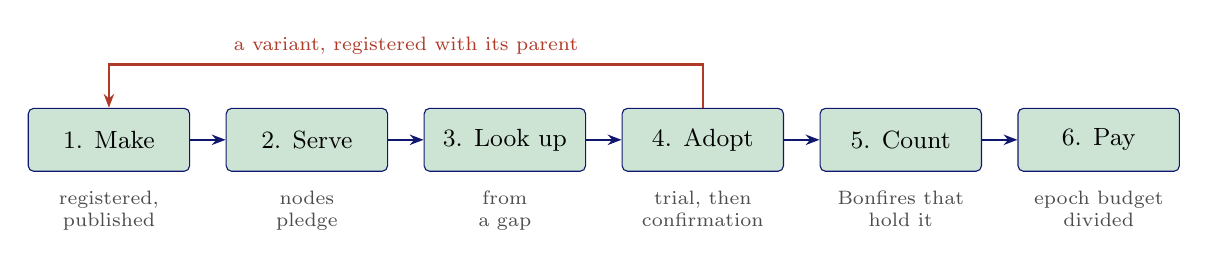
\begin{tikzpicture}[
  font=\small,
  stage/.style={draw=cxnnavy, fill=cxngreen, rounded corners=2pt, minimum width=2.05cm, minimum height=0.8cm,
               align=center},
  arr/.style={-{Stealth[length=5pt]}, thick, cxnnavy},
  note/.style={font=\scriptsize, text=black!70, align=center}
]
  \node[stage] (pub) {1. Make};
  \node[stage, right=0.45cm of pub] (ado) {2. Serve};
  \node[stage, right=0.45cm of ado] (enc) {3. Look up};
  \node[stage, right=0.45cm of enc] (chk) {4. Adopt};
  \node[stage, right=0.45cm of chk] (rep) {5. Count};
  \node[stage, right=0.45cm of rep] (set) {6. Pay};
  \draw[arr] (pub) -- (ado);
  \draw[arr] (ado) -- (enc);
  \draw[arr] (enc) -- (chk);
  \draw[arr] (chk) -- (rep);
  \draw[arr] (rep) -- (set);
  \node[note, below=0.12cm of pub] {registered,\\published};
  \node[note, below=0.12cm of ado] {nodes\\pledge};
  \node[note, below=0.12cm of enc] {from\\a gap};
  \node[note, below=0.12cm of chk] {trial, then\\confirmation};
  \node[note, below=0.12cm of rep] {Bonfires that\\hold it};
  \node[note, below=0.12cm of set] {epoch budget\\divided};
  \draw[arr, modelred] (chk.north) -- ++(0,0.55) -| node[pos=0.25, above, font=\scriptsize, text=modelred]
    {a variant, registered with its parent} (pub.north);
\end{tikzpicture}

\caption{The life of a construction. Members' discourse yields it and their Bonfire registers and publishes it;
nodes pledge to the Bonfire and serve it; another Bonfire's gap becomes a lookup; the construction is tried and
adopted; each epoch the Bonfires that hold it are counted; the epoch budget is divided. A Bonfire that changes it
registers a variant with its parent.}\label{fig:life}
\end{figure}

\section{Adoption}\label{sec:adoption}

A construction made in one Bonfire becomes part of another's language by the route a word takes between people.
Someone meets a form they cannot read, learns it from a source that can, and keeps it if it goes on working. The
protocol gives that route five steps; Figure~\ref{fig:adoption} shows the route.

\paragraph{Signal.} Each Bonfire publishes, with its grammar, a signal: a statement of what the grammar is for.
Signals are how a grammar is found. They cost nothing to make, so a Bonfire could claim every purpose; for that
reason no payment rests on a signal, and each Bonfire ranks the grammars it consults by its own record of which
ones answered it.

\paragraph{Lookup.} When a Bonfire's agent meets a form its inventory cannot read, the gap becomes a \emph{lookup}:
a query to the network, routed by the signals into the grammars of other Bonfires. Published grammars are open, so
the lookup runs on a node that serves the asking Bonfire, which fetches the foreign grammar and applies it. The text that
could not be read is shown to nobody else. Lookups that no grammar answers, grouped by what they were about, are
the network's record of what remains to be structured.

\paragraph{Trial.} If a foreign grammar reads the text, the constructions necessary to that reading are on offer
together, since a construction torn from those it depends on may read nothing. They enter the asking Bonfire's
inventory by reference to their originator's registration, at the starting score, as a \emph{trial}. A construction
on trial reads, and its effect is switched off: an effect taken from elsewhere is behaviour taken from elsewhere,
and it should not act before someone in the Bonfire has agreed to it.

\paragraph{Selection.} Over the Bonfire's later discourse a construction on trial succeeds or fails beside the
Bonfire's own, and its standing moves by the rule of Section~\ref{sec:constructions}. Where several Bonfires offer
a reading for the same gap, their constructions compete here, and different Bonfires may settle differently. This
is the naming game, played between communities \citep{steels1995spatial,baronchelli2006sharp}.

\paragraph{Adoption.} The Bonfire's stakeholders confirm a construction that has earned its place, and it stays in the Bonfire's inventory with its effect on. It does not become one of the Bonfire's own
constructions: its originator is unchanged. The confirmation is a signed attestation that references the
originator's registration; that act is the \emph{adoption}. From then on, a Bonfire \emph{holds} a construction in
an epoch when it has adopted it and the construction did necessary work in that Bonfire's own discourse in the
epoch, as shown by receipts that anyone can re-execute. Holding is what the protocol counts
(Section~\ref{sec:reward}).

Adoption is free, and it is pulled by need: no Bonfire can place a construction in another. A Bonfire that starts
from nothing becomes useful by adopting, and it has a reason to adopt by reference instead of copying, since a
reference brings the construction as its originator maintains it and a copy earns its copier nothing
(Section~\ref{sec:lineage}). A group that begins from the whole of another Bonfire's grammar is in this sense not a
rival to it: it is one more community that holds its constructions.

\begin{figure}[!htb]
\centering
% fig:adoption -- a gap in B, a lookup into A's grammar, trial and adoption, and what flows back to A
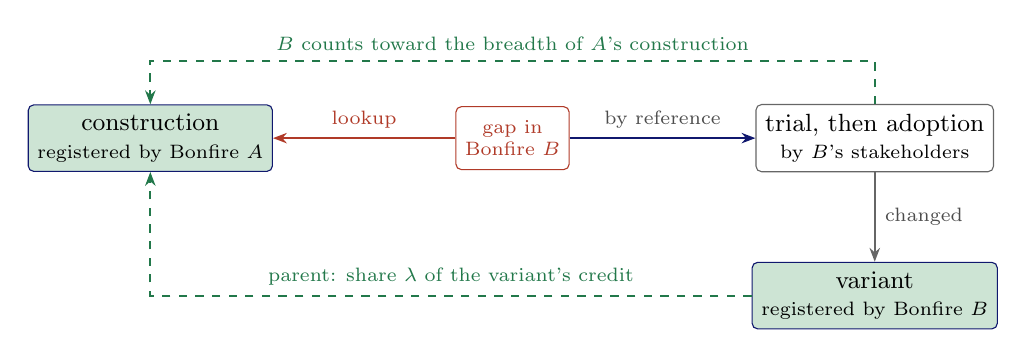
\begin{tikzpicture}[
  font=\small,
  cxn/.style={draw=cxnnavy, fill=cxngreen, rounded corners=2pt, minimum width=3.0cm, minimum height=0.8cm,
              align=center},
  plain/.style={draw=black!60, rounded corners=2pt, minimum width=3.0cm, minimum height=0.8cm, align=center},
  desc/.style={-{Stealth[length=5pt]}, thick, cxnnavy},
  credit/.style={-{Stealth[length=5pt]}, thick, okgreen, dashed},
  note/.style={font=\scriptsize, text=black!70, align=center}
]
  \node[cxn] (pa) at (0,0) {construction\\[-1pt]{\scriptsize registered by Bonfire $A$}};
  \node[draw=modelred, text=modelred, rounded corners=2pt, minimum height=0.8cm, align=center, font=\scriptsize]
    (gap) at (4.6,0) {gap in\\Bonfire $B$};
  \node[plain] (ad) at (9.2,0) {trial, then adoption\\[-1pt]{\scriptsize by $B$'s stakeholders}};
  \node[cxn] (var) at (9.2,-2.0) {variant\\[-1pt]{\scriptsize registered by Bonfire $B$}};
  \draw[desc, modelred] (gap) -- node[above, font=\scriptsize, text=modelred] {lookup} (pa);
  \draw[desc] (gap) -- node[above, font=\scriptsize, text=black!70] {by reference} (ad);
  \draw[desc, black!60] (ad) -- node[right, font=\scriptsize, text=black!70] {changed} (var);
  \draw[credit] (ad.north) -- ++(0,0.55) -| node[pos=0.25, above, font=\scriptsize, text=okgreen]
    {$B$ counts toward the breadth of $A$'s construction} (pa.north);
  \draw[credit] (var.west) -| node[pos=0.25, above, font=\scriptsize, text=okgreen]
    {parent: share $\lambda$ of the variant's credit} (pa.south);
\end{tikzpicture}

\caption{Adoption. A form from Bonfire $A$ meets a gap in Bonfire $B$. $B$'s lookup finds $A$'s construction, tries
it, and adopts it; $B$ then counts toward the breadth of $A$'s construction for as long as $B$ holds it. If $B$
changes the construction it registers a variant with $A$'s as its parent, and a share $\lambda$ of the variant's
credit passes to $A$.}\label{fig:adoption}
\end{figure}

\section{Lineage}\label{sec:lineage}

A construction that is adopted is often changed, and a new construction is seldom made from nothing. The protocol
records that history as \emph{lineage} and moves credit, defined in Section~\ref{sec:reward}, along it.

\paragraph{Variation.} A Bonfire that specialises, generalises or combines constructions that exist, its own or
another's, registers the result as a new construction. Those it was made from are its \emph{parents}, and they are
declared when it is registered. In language-game experiments with FCG, agents acquire constructions in this way,
through interaction, by reading the other's intention and finding patterns in what they already hold
\citep{nevens2022language}.

\paragraph{Origin.} The Bonfire that registers a construction is its originator. Two Bonfires may register one
jointly, and it is then credited to both in equal parts: equal by rule, not by measurement, so that neither has
anything to gain from disputing how much it contributed.

\paragraph{Credit along a lineage.} Two rules move credit between a construction and its ancestors.

\emph{A copy earns nothing.} A construction is credited only for what could not have been read without it, and this
is tested on the meaning, not on the form. Anyone may show an earlier registration with which the same text would
have received the same reading. The credit then belongs to the earlier registration. A construction registered
under a new hash or a renamed form that does what an earlier one already did therefore earns nothing, whether or
not it declared a parent. Priority belongs to the first to register. Use is open to all, and credit is what is
exclusive.

\emph{A descendant pays its parents.} A fixed share $\lambda$ of the credit a construction earns passes to the
parents it declares, and from them to theirs. A construction that few hold directly, but on which much is built,
is paid through what is built on it. This is the rule intended to fund foundational work, and to make use yield
the material for further structure. It reaches only parents that are declared. Declaring a parent gives up credit,
and beyond the copy rule nothing yet compels it (Section~\ref{sec:open}).



\section{Reward}\label{sec:reward}

At the end of each epoch the epoch budget is divided among Bonfires according to how widely the constructions they
originated are held by other Bonfires, and each Bonfire divides what it receives between the nodes that serve it
and its stakeholders.

\paragraph{Breadth.} The \emph{breadth} of a construction in an epoch is the number of Bonfires that hold it
(Section~\ref{sec:adoption}), counting only Bonfires that are independent of its originator and of one another and
that carry at least a minimum bond (Section~\ref{sec:bond}). A Bonfire counts once in an epoch however often it
used the construction, and it counts again in every later epoch in which it still holds it. Use inside the
originating Bonfire counts nothing: a community needs no payment for work it does for itself.

\paragraph{Credit.} A construction's \emph{credit} in an epoch depends only on its breadth. Below a threshold
breadth it is nothing, and above the threshold it rises with breadth. Writing $n$ for the breadth, $n_0$ for the
threshold and $g$ for the rule,
\begin{equation}\label{eq:credit}
  \text{credit} \;=\; g(n), \qquad g(n) = 0 \ \text{ for } n < n_0, \qquad g \text{ increasing for } n \ge n_0 .
\end{equation}
The threshold is what makes a small group's agreement worth nothing. Two Bonfires that adopt each other's
constructions, or one Bonfire that registers ten thousand constructions which a single partner holds, sit below it.
The shape of $g$ above the threshold is left open (Section~\ref{sec:open}). A share $\lambda$ of a construction's
credit passes to the parents it declares (Section~\ref{sec:lineage}), and a Bonfire's credit is the sum over the
constructions it originated, after those transfers.

\paragraph{Why holding, and not spread.} A construction is paid for lasting in other communities, and nothing is
paid for passing it on. That a convention is taken up does not show that it carries knowledge: among the early
users of a new term, short-lived fashions and lasting changes look alike \citep{tarrade2024position}. A construction that is tried and dropped stops counting when it is dropped. One that a
community keeps is counted afresh each epoch, so a grammar that stays in use keeps being funded. Counting each
Bonfire once also makes repetition worthless. A finding about words points the same way: over short periods, a
word's spread across users and threads predicts its fate better than its frequency does
\citep{altmann2011niche}.

\paragraph{Failure.} A failed reading counts for nothing, and it lowers the standing of the constructions tried
(Section~\ref{sec:constructions}), so a construction pushed into contexts where it does not work leaves that
inventory. Failures are never subtracted from an originator's credit. If they were, a Bonfire could harm another
by adopting its constructions and misusing them.

\paragraph{Division.} A fixed fraction of the epoch budget is set aside to pay for spot checks
(Section~\ref{sec:bond}). The rest is divided among Bonfires in proportion to credit, and each Bonfire's payment is
capped by the ceiling of Section~\ref{sec:bond}. The Bonfire passes a share $s$ of its payment to the nodes pledged
to it, equally, and the rest goes to its stakeholders. The Bonfire publishes $s$. Bonfires compete for nodes
through this rate, so the split between those who structure and those who serve is set by the participants.

\paragraph{From contribution to stake.} A registration names the members whose contributions yielded the
construction: those who taught it, and those who confirmed it. Of the stakeholders' part of what the construction earns, a fraction published by the Bonfire vests to them
as stake in that Bonfire. A member who arrives with nothing and whose words become
constructions that other communities keep thereby becomes a stakeholder. This is the protocol's answer to how
people who take part in making sense of something come to hold a share of what is made.

\paragraph{A worked epoch.} As a thought experiment, let $n_0 = 3$ and, for illustration only, $g(n) = n - 2$ at
or above the threshold. Let $\lambda = 0.1$, the ceiling rate $c = 0.01$ and each node's pledge $q = 10{,}000$ (Section~\ref{sec:bond}), and $s = 0.4$, with $1{,}000$ left of the epoch budget after spot checks. Bonfire $A$ originated $x$, held by six
Bonfires, and $y$, held by two; five nodes are pledged to it. Bonfire $B$ originated $z$, a variant of $x$ held by
four Bonfires; four nodes are pledged to it. Table~\ref{tab:epoch} follows the division.

\begin{table}[!htb]
\centering\small
\begin{tabular}{@{}lrr@{}}
\toprule
 & \textbf{Bonfire $A$} & \textbf{Bonfire $B$} \\
\midrule
Credit from breadth & $x$: $4$, \ $y$: $0$ & $z$: $2$ \\
After the lineage share ($0.2$ from $z$ to $x$) & $4.2$ & $1.8$ \\
Share of $1{,}000$ in proportion to credit & $700$ & $300$ \\
Ceiling, $c\,k\,q$ & $500$ & $400$ \\
Paid & $500$ & $300$ \\
\quad to nodes (share $s$) & $200$ & $120$ \\
\quad to stakeholders & $300$ & $180$ \\
\bottomrule
\end{tabular}
\caption{A worked epoch (thought experiment). The $200$ that Bonfire $A$'s ceiling does not admit is not paid;
what becomes of it is a question of issuance, left to the token model. Construction $y$, held by two Bonfires,
earns nothing.}\label{tab:epoch}
\end{table}

\section{Stake}\label{sec:bond}

The rules of Section~\ref{sec:reward} decide what breadth is worth. They do not decide whose word is taken that
the Bonfires holding a construction are separate parties. That is the work of stake.

\paragraph{Bond and pledge.} The stake its stakeholders hold in a Bonfire is the Bonfire's \emph{bond}.
Stakeholders share in the Bonfire's payment by its own rule, weigh in what enters its grammar, and lose their stake
if the Bonfire is found at fault: they underwrite it, as the masters of a guild answered for its mark. A Bonfire
counts toward the breadth of other Bonfires' constructions only while its bond is at least a minimum, $m$. A node
that serves a Bonfire commits to it a \emph{pledge} of a fixed size, $q$. Stake pledged to one Bonfire cannot be
pledged to another, so where a node places its pledges is a choice with a cost. Because every pledge is the same
size, an operator who runs many nodes has committed many pledges, and the number of nodes behind a Bonfire is a
measure of the stake committed to serving it.

\paragraph{The ceiling.} Stake is the accountability engine of the protocol. It makes a Bonfire and a node
answerable, and it limits what can be earned; it adds nothing to credit. In one epoch a Bonfire is paid at most a
fixed multiple of the pledges committed to it. Writing $k$ for the number of nodes pledged to the Bonfire, $c$ for
the multiple, the \emph{ceiling rate}, and $e$ for what the Bonfire is paid in the epoch,
\begin{equation}\label{eq:ceiling}
  e \;\le\; c\,k\,q .
\end{equation}
Breadth fills the ceiling, and the nodes committed to serving a grammar set it: uptake by other communities is the
demand, and committed capacity is the limit. A pledge earns nothing of itself. The ceiling is linear in the number
of pledges, so dividing or combining nodes changes nothing. A new Bonfire serves itself, and its ceiling is set by its own pledge. Pledges move toward grammars whose breadth earns more than their ceilings admit, and away from those that
cannot fill them, so capital follows uptake and does not direct it. An amount above a ceiling is not paid; what
becomes of it is a question of issuance, left to the token model. The reason for a ceiling and not a weight is
empirical: where stake has raised rewards directly, rewards have followed stake and not service
(Section~\ref{sec:prior}).

A node receives its part of the share $s$, so the most a pledge can yield is $s\,c$ per epoch.

\paragraph{Faults.} Table~\ref{tab:faults} lists what stake answers for.

\begin{table}[!htb]
\centering\small
\begin{tabularx}{\textwidth}{@{}p{0.34\textwidth}p{0.30\textwidth}X@{}}
\toprule
\textbf{Fault} & \textbf{What is lost} & \textbf{How it is decided} \\
\midrule
A receipt that does not re-execute, a receipt withheld on challenge, or a commitment altered after the fact &
The pledge of the node that signed it &
Re-execution by any node; a disagreement is settled by a bonded vote of nodes \\
\addlinespace
One party posing as several Bonfires, so that its own constructions appear widely held &
The bonds of the Bonfires found to be one party, and the pledges of the nodes that party runs &
A judged challenge, settled by a bonded vote \\
\bottomrule
\end{tabularx}
\caption{Faults, what is lost, and how each is decided.}\label{tab:faults}
\end{table}

The first kind of fault is a matter of computation. One honest node suffices to find it, since re-execution has one right answer where the engine is deterministic. A ledger does not run the grammar engine, however, so when the accused node disputes the finding the
dispute goes to a vote of nodes weighted by stake, and the vote is sound while most of the voting stake is honest.
The second kind cannot be settled by computation at all. The question put to the vote is narrow: whether the
governing stake of several Bonfires is controlled by one party. Each real Bonfire has a history to show for
itself, in its members, its own constructions, its gaps, trials and adoptions. Because the protocol is indifferent
to who or what produced a piece of discourse, generated conversation is not a fault. The design of the judged vote
is among the open problems of Section~\ref{sec:open}.

One further rule is proposed and left open. When a Bonfire is found at fault, the nodes pledged to it that the
party at fault does not run lose a part of their pledge. Whoever's capital is exposed is who checks, and a node
that can lose by serving a sham has a reason to examine a Bonfire before pledging to it. The cost is that an
honest node can lose stake through another's fraud, and that nodes will be slow to serve a Bonfire with no history.

A fraction $\varphi$ of slashed stake pays the challenger and the rest is destroyed. If the whole of it went to the
challenger, an owner could challenge its own parties through another identity and lose nothing. Spot checks are
paid from the part of the epoch budget set aside for them, whether or not they find a fault; this, and not the
slash, is what answers the difficulty of Section~\ref{sec:agreements} that unpaid checks are not carried out.

\paragraph{Lock.} A scientist's stake in a claim is reputation, which is slow to build and cannot be lent. A token
can be borrowed for a day. Stake is therefore locked for a period at least as long as a challenge takes to bring,
and whoever has asked to withdraw remains liable for faults committed while the tokens were locked.

\section{Security}\label{sec:security}

\begin{proposition}\label{prop:service}
To earn under the protocol, a Bonfire must originate constructions that at least $n_0$ independent Bonfires adopt
and go on holding, or constructions from which such constructions are declared to descend. A party that wants to
earn without that must make its constructions appear widely held. Where it does so by posing as several Bonfires,
it commits a fault, and under the assumptions and limits below what it can earn is bounded by the stake it puts at
risk.
\end{proposition}

The argument rests on four assumptions: (1)~the host chain orders registrations and commitments honestly; (2)~every
receipt is open to challenge, a random sample is spot-checked, at least one of the nodes that examine a receipt is
honest, and most of the stake that votes on a dispute is honest; (3)~the text of an encounter is available to a
node that samples or challenges its receipt; (4)~one party posing as several Bonfires is challenged and slashed
with probability at least $p$ in each epoch.

\paragraph{Attacks.} Table~\ref{tab:attacks} lists the ways of seeking payment without providing the service, with
the rule that answers each.

\begin{table}[!htb]
\centering\small
\begin{tabularx}{\textwidth}{@{}p{0.38\textwidth}X@{}}
\toprule
\textbf{Attack} & \textbf{What answers it} \\
\midrule
Repeating a use, or inventing members & A Bonfire counts once per epoch toward a construction's breadth
(Section~\ref{sec:reward}) \\
A Bonfire using its own grammar & Use inside the originating Bonfire counts nothing \\
A few Bonfires adopting one another's constructions & Breadth below the threshold $n_0$ earns nothing \\
Registering many constructions & Each needs its own breadth \\
Copying a construction, or renaming its form & Credit belongs to the earliest registration that gives the same
reading (Section~\ref{sec:lineage}) \\
Adopting a construction in order to misuse it & Failures are never subtracted from credit \\
Signing a false receipt & Re-execution by an honest node, a vote if disputed; the pledge is lost
(Section~\ref{sec:bond}) \\
Challenging oneself to recover stake & Only a fraction $\varphi$ of a slash reaches any challenger \\
Borrowing stake for a day & The lock \\
One party posing as several Bonfires & Bounded by the ceiling, the bonds and the chance of challenge (below) \\
Paying independent Bonfires to hold a construction & Open (Limits) \\
Many independent Bonfires agreeing to hold one another's constructions & Accepted. The threshold sets how many must agree; where it should sit is open \\
A committed minority capturing a convention & Accepted. The network agrees on a ledger, not on one language
(Section~\ref{sec:prior}) \\
\bottomrule
\end{tabularx}
\caption{Attacks and the rules that answer them.}\label{tab:attacks}
\end{table}

The last four rows are not answered by a rule. Two are accepted and one is open. Posing as several Bonfires is
bounded, and the rest of this section is about it.

\paragraph{Posing as many.} A party that wants breadth it has not earned must supply the Bonfires itself. It founds
at least $n_0$ of them, bonds each, has them adopt the constructions of a Bonfire it also controls, and generates
discourse in each so that the constructions do necessary work there. Every receipt re-executes, because the
computations are real. Nothing in a receipt shows who controls a Bonfire.

What limits the arrangement is stated first in words. Each sham Bonfire must carry the minimum bond. The
originating Bonfire is paid only up to its ceiling, so the party must also commit the pledges that set it. Holding
all of that stake has a cost. In every epoch all of it may be lost, and an owner who brings the challenge itself
recovers only the challenger's fraction. So the income from posing as many is at most a multiple of the capital put
at risk, and that multiple can be set below the cost of the risk.

Let $r$ be the cost of capital per epoch, the return given up by locking a token; $p$ the probability of
assumption~4; and $\varphi$ the challenger's fraction. A party that poses as $n_0$ Bonfires and serves its
originating Bonfire with $k$ nodes of its own is paid at most $c\,k\,q$ in an epoch, keeping both the nodes' share
and the stakeholders'. Its stake is $n_0\,m + k\,q$, which costs $r\,(n_0 m + k q)$ to hold and is exposed to an
expected loss of $(1-\varphi)\,p\,(n_0 m + k q)$. It does not profit when
\[
  c\,k\,q \;\le\; \bigl(r + (1-\varphi)\,p\bigr)\,(n_0\,m + k\,q),
\]
for which it is enough that $c \le r + (1-\varphi)\,p$. An honest node whose Bonfire fills its ceiling earns
$s\,c\,q$ on a pledge that costs $r\,q$ to hold, and profits when $s\,c > r$. The protocol and the published shares
must therefore satisfy
\begin{equation}\label{eq:ring}
  \frac{r}{s} \;<\; c \;\le\; r + (1-\varphi)\,p ,
\end{equation}
with a margin on the right. The window is not empty only if $r\,(1-s)/s < (1-\varphi)\,p$, which sets a least
share that a Bonfire must pass to its nodes. The ceiling rate sits high enough that serving pays a node its cost of capital, and no
higher than that cost plus the chance of being caught, discounted by what a challenger can recover. The bonds of
the sham Bonfires are a further cost that does not depend on being caught: below a certain scale they exceed
anything the ceiling admits.

The same reasoning covers an honest Bonfire that serves itself, has room under its ceiling and is tempted to
add sham holders. What it could gain is at most what the ceiling admits, and what it exposes is its own bond as
well as the sham bonds and its pledges.

The bound uses the following and nothing else. (a)~The ceiling and the minimum bond are enforced. (b)~A successful
challenge takes the whole of the stake listed in Table~\ref{tab:faults}. (c)~Of slashed stake at most $\varphi$
reaches any challenger and the rest is destroyed. (d)~The cost of capital is $r$ for all parties, and they are
neutral to risk. (e)~An honest party is not slashed by mistake. (f)~$p$ is a floor that holds from the first
epoch. The bound is on capital, not on the number of identities: every Bonfire that counts is bonded and every
pledge is the same size, so dividing capital among more Bonfires or nodes raises nothing.

\paragraph{Limits.}
\begin{itemize}
  \item The bound depends on $p$, which is unmeasured (Section~\ref{sec:open}). It is also not a given: it is the
  result of someone looking. The parties with a reason to look are challengers, paid the fraction $\varphi$, and
  nodes whose pledges would be exposed under the rule proposed in Section~\ref{sec:bond}. If faking is rare,
  looking pays little, and a protocol cannot assume that $p$ stays where it was measured.
  \item The bound assumes that the party supplies the nodes itself. If honest nodes pledge to a Bonfire whose breadth
  is a sham, they set its ceiling while only the sham bonds are certainly at risk. The case then rests on whether
  those nodes can lose their pledges, which is left open.
  \item Breadth can be bought. A Bonfire that holds a construction earns nothing by it and needs one reading an
  epoch to do so, so an originator can pay independent Bonfires, outside the protocol, to hold what they do not
  need. No rule answers this. It costs what $n_0$ holders ask, which is a reason for a threshold that is not small.
  \item The evidence that several Bonfires are one party is their histories, and it is a matter of judgement.
  Deciding it reintroduces opinion at one point of the protocol.
  \item While stake is locked its holding cost is already paid. A party with stake it cannot yet withdraw is surely deterred only if $c < (1-\varphi)\,p$, which is stricter than (\ref{eq:ring}). The lock should be no longer than
  challenges require.
  \item The epoch budget is shared. Faked breadth that only breaks even still takes income from honest parties,
  which is why the right-hand inequality needs a margin.
  \item A reward that rises with breadth, from a threshold, favours what is already widely held, and a
  construction of real use to two communities earns nothing.
  \item The operating cost of a node is outside the condition. A node that serves real discourse spends more than
  one that serves generated discourse.
  \item The comparison with earlier systems is a hypothesis: none of them paid on replayable use
  (Section~\ref{sec:prior}).
\end{itemize}

\section{Relation to prior institutions and systems}\label{sec:prior}

\paragraph{The guild.} The craft guilds of preindustrial Europe are the nearest historical model for an institution
that holds and transmits working knowledge, and historians disagree about them in an instructive way. On one
account guilds existed to provide transferable skills through apprenticeship, and they spread technique through
migrant labour \citep{epstein1998craft}. On another they excluded competitors, manipulated markets, blocked
innovations and denied apprenticeships to outsiders, to the benefit of their members and of political elites
\citep{ogilvie2019guilds}. Both accounts describe one institution, and we read them together as follows: a guild
could pay for the keeping of knowledge only out of the returns of exclusion. A Bonfire keeps the first function and
has no need of the second. It is paid from issuance for what other communities take up, so it gains by publishing
and loses nothing when anyone uses what it publishes. Membership is open as well. What a guild's master held by
admission, a Bonfire's stakeholder holds by work: stake is earned through contribution.

\paragraph{Issuance that follows opinion, stake or volume.} Bittensor allocates by the scores
validators assign to one another's work, combined by stake. An empirical study of 64 of its sub-networks found that
validators' rewards tracked their stake, with correlations between $0.80$ and $0.95$, while miners' rewards tracked
measured performance only weakly, between $0.10$ and $0.30$ \citep{lui2025bittensor}, and the project's own
documentation states that a validator who copies the expected consensus can earn more per unit of stake than one who
evaluates honestly \citep{bittensor2026weightcopy}. The closest existing design is The Graph. Developers publish
data definitions, staked indexers serve them, and an indexer's signed attestation of a query response can be
disputed and re-run by an arbitrator \citep{thegraph2026docs}. Its issuance, however, follows stake and not use:
indexing rewards are distributed in proportion to the signal curators place on a definition and the stake indexers
allocate to it. The project itself reports that neither quantity measures whether an indexer served a query, that
15.2\% of indexing rewards in 2025 went to indexers that were not delivering value, and that it has added an
eligibility test based on queries served \citep{thegraph2026eligibility}. Where staked votes alone direct emissions,
as with Curve's gauge weights \citep{curve2026gauges}, markets have formed in which those votes are bought
\citep{votium2026docs}. And a marketplace that rewarded reported trading volume saw the volume manufactured: almost
80\% of the wash-trading operations identified on LooksRare closed at a profit \citep{lamorgia2023nft}. These are
the reasons the second agreement is reached by re-execution, where there is nothing to copy; that stake is a
ceiling and not a weight; and that what fills the ceiling is breadth and not volume.

\paragraph{Paying on speech and attention.} Several systems have attached payment to posts or to persons.
Friend.tech let users buy ``keys'' in individuals; it collected almost \$90 million in fees, and its daily fees,
which once reached \$2 million, stood below \$100 by September 2024 \citep{craig2024friendtech}. On Steemit, where
stake-weighted votes on posts directed rewards, more than 16\% of transfers went to accounts suspected of being bots
that sold votes \citep{li2019steem}. On Farcaster, token rewards raised the volume of posting while often failing to
raise, and sometimes lowering, its quality, and 92.4\% of the tipping transactions of one token came from two bot
accounts \citep{yang2025farcaster}. In all three the quantity paid on was a proxy at the level of the person or the
post, and in the last two the proxy was produced by bots. We draw a
narrow conclusion: a use that a third party can re-execute is a different kind of evidence from a vote, a price or a
tip, and it still needs a defence against one party posing as many. For the same reason the protocol pays nothing for
passing a construction on. A reward for transmission is a reward for attention, and it is paid before anyone knows
whether what spread was kept.

\paragraph{One ledger, many languages.} A protocol built on naming games might be expected to drive its
participants toward a single shared language. The literature suggests otherwise. On networks with strong community
structure, naming games settle into clusters that keep different conventions for long periods, in some cases
indefinitely \citep{lu2009naming,dallasta2006nonequilibrium}. A convention can also be captured by a small committed
group: on a complete graph, a committed minority of about 10\% changes the time to consensus from exponential in the
population to logarithmic \citep{xie2011social}. Populations of language-model agents form conventions in
the same way \citep{ashery2025emergent}. We take this to mean that agreement on meaning is neither stable enough nor
secure enough to carry payment. The protocol asks for agreement only on the ledger, and meaning stays plural: breadth counts the communities that
hold a construction and does not require that all of them do.

\paragraph{A studied system of discrete rules.} Collectible card games are a studied case of a population using
discrete rules with definite effects: the cards of one such game are rules precise enough that the game has been
shown to be Turing complete \citep{churchill2021magic}, and what a card contributes depends on what it is combined
with \citep{kritz2025synergy}. The cards trade in a real market \citep{luckingreiley1999magic}, in which cards
designated rare sell for more than functionally equivalent substitutes \citep{hughes2022rarity}. That market
prices scarcity over and above function. A protocol built on open use has no scarcity of that kind to price. What
is scarce in it is credit for having been first (Section~\ref{sec:lineage}).

\paragraph{The scientific process.} Science rewards the structuring of knowledge so that its use produces more of
it, and it is the working precedent for open use with exclusive credit. A result is free to use, and what its
author holds is priority and citation, the counterparts here of registration and lineage. 

\section{Open problems}\label{sec:open}

\begin{itemize}
  \item \emph{Determinism.} Replay requires that the same engine, inventory and search order give the same reading
  on every machine. This has not been measured. Where implementations differ, a dispute has no right answer; The
  Graph resolves such cases as a draw \citep{thegraph2026docs}.
  \item \emph{The shape of the reward.} Where the threshold $n_0$ sits and how credit rises above it. A low
  threshold admits small groups; a steep rise favours what is already widely held.
  \item \emph{The value of $p$.} Condition (\ref{eq:ring}) can be met only if the chance that one party posing as
  several Bonfires is caught is known to within a margin, and stays there when few are looking.
  \item \emph{Deciding a judged challenge.} Who votes, what a challenger must post, and what a mistaken slash costs
  an honest party. The argument of Section~\ref{sec:security} assumes mistaken slashes are rare.
  \item \emph{Nodes behind a Bonfire at fault.} Whether, and in what part, a node loses its pledge when the Bonfire
  it serves is found at fault (Section~\ref{sec:bond}).
  \item \emph{Parameters.} The ceiling rate $c$, the pledge $q$, the minimum bond $m$, the challenger's fraction
  $\varphi$, the lineage share $\lambda$, the length of the lock, the rate of spot checks and what they are paid,
  and whether the protocol bounds the share $s$.
  \item \emph{Necessity and granularity.} A reading may survive the removal of either of two constructions and fail
  without both; the test then credits neither. Attribution rules of the Shapley kind would handle this but are
  vulnerable when a participant can appear under more than one name \citep{ohta2008anonymity}.
  \item \emph{Comparing meanings.} The copy rule asks whether an earlier construction gives the same reading. A copy
  that renames the symbols of the meaning gives a different one, and a test of equivalence is wanted.
  \item \emph{Registration in bulk.} Priority belongs to the first to register, and constructions can be generated
  and registered in any number ahead of the communities that would have made them. What registration should cost
  is open.
  \item \emph{Declaring parents.} A construction that declares a parent gives up a share of its credit. A test of
  derivation that anyone can run is wanted.
  \item \emph{The base grammar.} It earns nothing, and whoever changes it can make any construction unnecessary.
  Who maintains it, and how that work is paid for, is open.
  \item \emph{What a node costs.} A node is paid a share of issuance. Whether that covers the computation it
  supplies, and who pays where it does not, is open.
  \item \emph{Disclosure.} A challenge shows the turns of one encounter to the challenger.
  \item \emph{Payment from use.} The protocol is funded by issuance alone. Whether payment from those who use the
  work of agents further down the supply chain should stand behind it is open.
  \item \emph{Learning without teaching.} Constructions enter a grammar today by being taught. Deriving them from a
  group's discourse is a proposed experiment of the companion paper \citep{vera2026constructions}.
\end{itemize}

Most of these would be settled by simulation before deployment: a naming game among Bonfires that hold different
grammars, with lookups, adoptions and lineage recorded, and the same game with a party that poses as several
Bonfires, a group that agrees to hold one another's constructions, and a party that borrows stake.

\section{Conclusion}\label{sec:conclusion}

The objective was a protocol under which discourse becomes something of value to those who took part in it and to
their community. It needs a unit of knowledge whose use is a fact, and the construction is such a unit: where
applying it to a text is deterministic, a use can be re-executed by a stranger, and a network can pay without
paying for anyone's opinion. It needs also a measure of worth that a few parties cannot manufacture, and the
measure proposed is breadth: how many independent communities have taken a construction up and kept it.

The protocol follows from those two. Communities publish their grammars for open use and signal what they are for.
A community that cannot read something looks it up, tries what it finds, and adopts what goes on working.
Adoption is free and is never pushed. An originator is paid according to the breadth of its constructions, with
nothing below a threshold, and a share passes to the parents each construction declares. Membership is free, and
members whose contributions become constructions earn stake in what they made. Nodes supply computation, and the
stake they pledge sets a ceiling that only breadth can fill, so capital follows uptake.

What cannot be computed is whether the communities that hold a construction are separate parties. That is anchored
in stake. Under the assumptions of Section~\ref{sec:security}, the ceiling rate is set no higher than the cost of
capital plus the chance of being caught posing as many, and within that limit a community that wants to earn has
one course open: to make constructions that others, who owe it nothing, find they need and keep.


{\small\setlength{\bibsep}{2pt plus 1pt}
\bibliographystyle{plainnat}
\bibliography{refs}}

\appendix
\section{Glossary}\label{app:glossary}

{\footnotesize\begin{multicols}{2}\begin{description}[leftmargin=1.9cm, style=nextline, itemsep=-1pt, topsep=0pt]
  \item[Adoption] A Bonfire's signed confirmation of a construction taken from another, by reference to its registration.
  \item[Bond] The stake its stakeholders hold in a Bonfire.
  \item[Bonfire] A community with a grammar, which it publishes for open use.
  \item[Breadth] The number of independent, bonded Bonfires that hold a construction in an epoch.
  \item[Ceiling] The most a Bonfire can be paid in an epoch: the ceiling rate times the pledges committed to it.
  \item[Holds] A Bonfire holds a construction in an epoch when it has adopted it and it did necessary work there.
  \item[Lookup] A query that takes a gap to the grammars other Bonfires have published.
  \item[Member] Anyone who takes part in a Bonfire's discourse.
  \item[Node] An operator that supplies computation, issues receipts and re-executes those of others.
  \item[Pledge] The fixed stake a node commits to one Bonfire it serves.
  \item[Signal] A Bonfire's published statement of what its grammar is for.
  \item[Stakeholder] A member who holds stake in a Bonfire, earned through contribution or locked.
  \item[Trial] The state of a construction taken from another Bonfire before it is adopted: it reads, and its effect is off.
  \item[Uptake] The adoption and continued holding of a construction by Bonfires other than its originator.
\end{description}\end{multicols}}

\section{What is built today}\label{app:built}

The following exist in memory-kernel 2.0.1 \citep{memorykernel2026} and are described in the companion paper
\citep{vera2026constructions}: reading each message of a conversation with a construction grammar, with no
generative model call in the write path; constructions taught in conversation, compiled with no model and admitted
once their teacher confirms them; a tally for each construction of its uses that answered, failed or were refused
by the world; and a record of which construction replaced which. The score rule of
Section~\ref{sec:constructions} and the network of Bonfires and nodes are proposed by this paper.


\end{document}
